\chapter{Implementácia systému}

Z kapitoly \ref{vyber} vyšlo že Linode je najlepšia volba pre virtuálne prostredie na nasadaenie mojho malého e-shopu. Vytvrenie prostredie bolo jednoduché ako je možné vidiet na obrázkoch \ref{img:one} a \ref{img:two}.

\begin{figure}[ht!]
  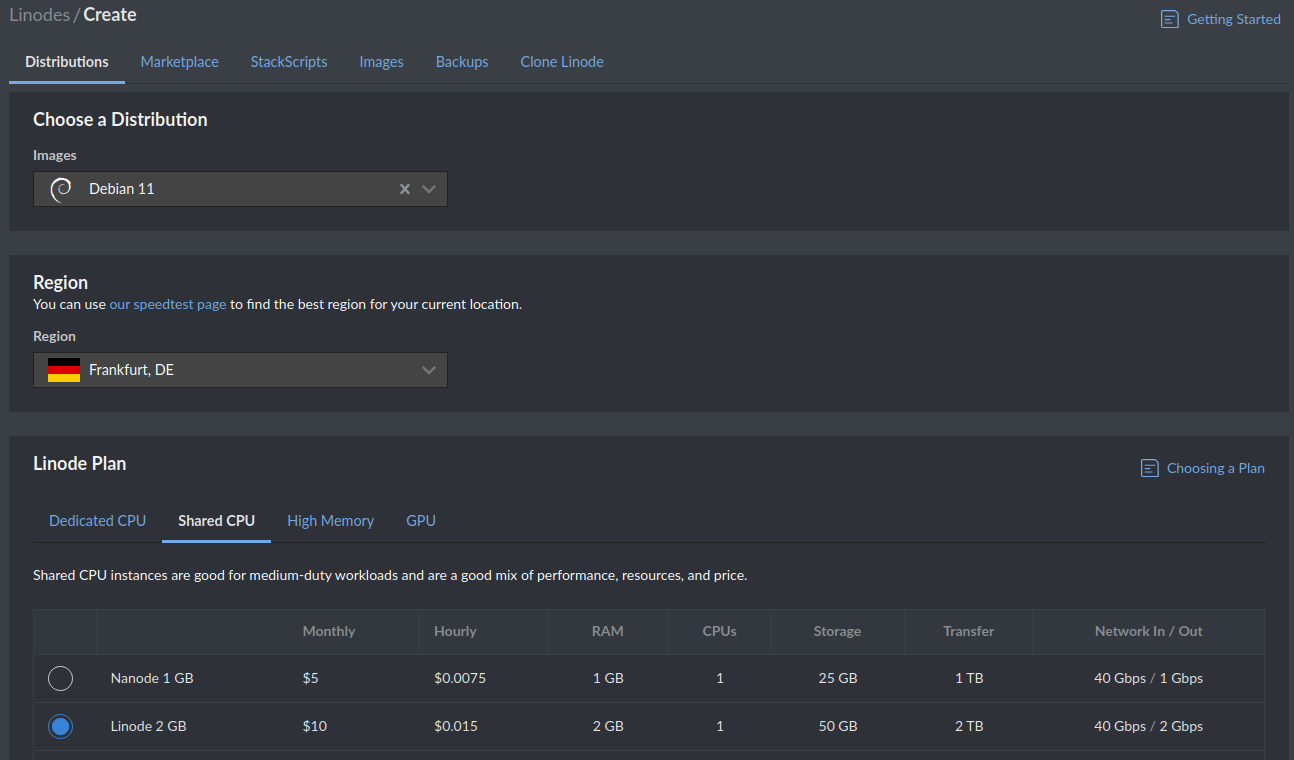
\includegraphics[width=\linewidth]{images/1.png}
  \caption{Prvá časť vytvorenia virtualného prostredia}
  \label{img:one}
\end{figure}

\begin{figure}[ht!]
  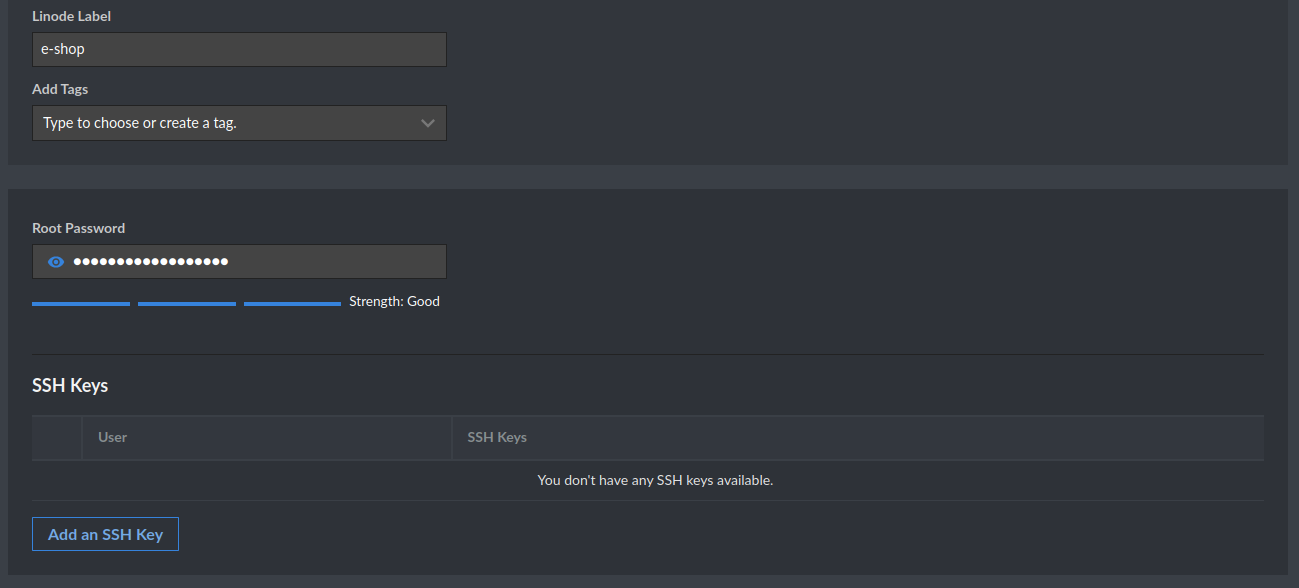
\includegraphics[width=\linewidth]{images/2.png}
  \caption{Druhá časť vytvorenia virtualného prostredia}
  \label{img:two}
\end{figure}

\noindent Uživatelské rozhranie ovládacieho panelu pre linode je velmi intuitívne a prehľadné ako je zase možné vidieť na obrázkoch \ref{img:three} a \ref{img:four}.

\begin{figure}[ht!]
  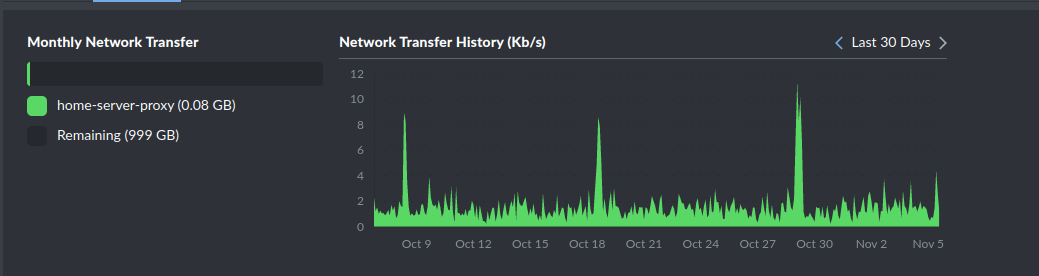
\includegraphics[width=\linewidth]{images/3.png}
  \caption{Prehľad sieťového provozu}
  \label{img:three}
\end{figure}

\begin{figure}[ht!]
  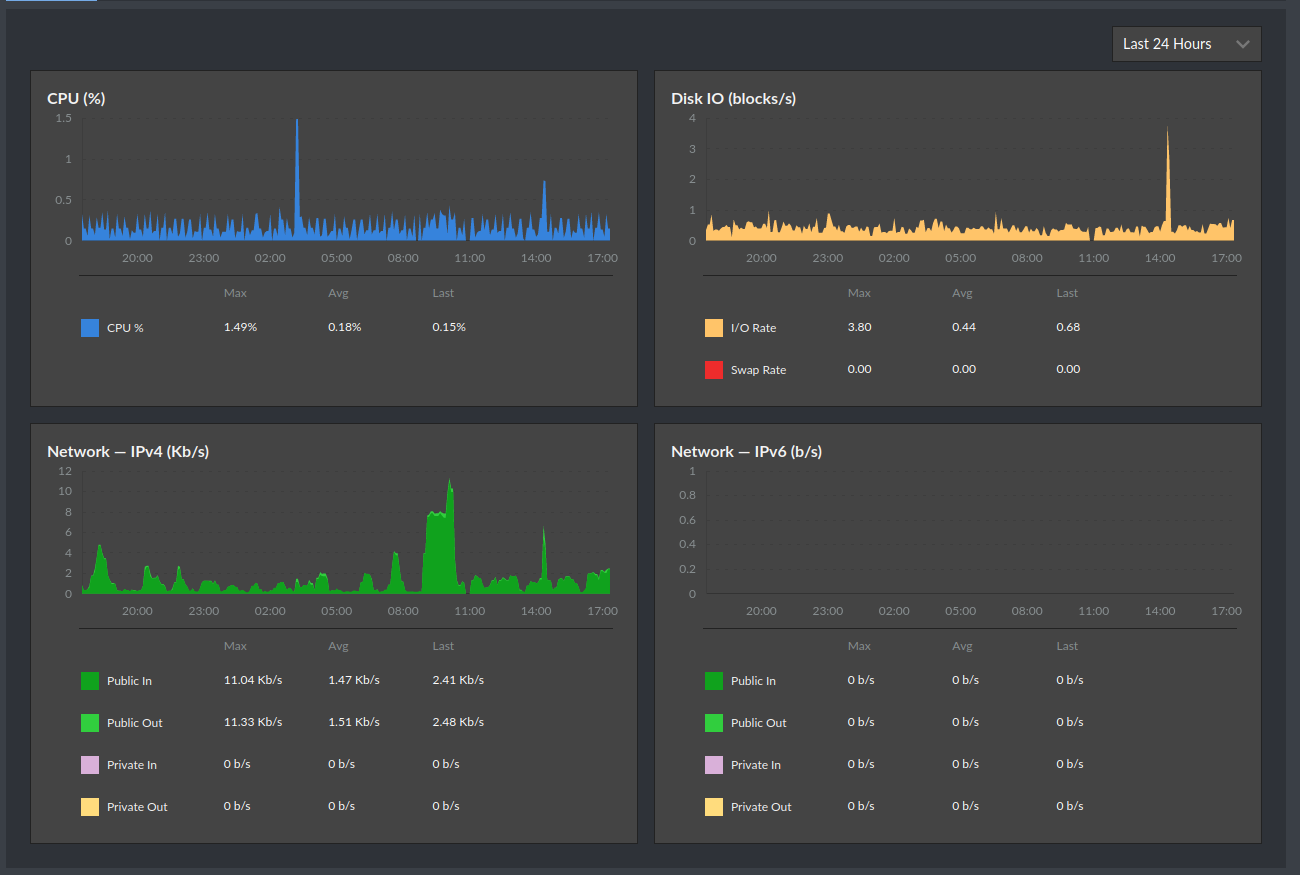
\includegraphics[width=\linewidth]{images/4.png}
  \caption{Prehľad systému}
  \label{img:four}
\end{figure}

Ako operáčný systém zvolím Linux Debian keďže mám skúsenosti s týmto operačným systémom a je na ňom jednoduchšie vytvárať a hostovať webové aplikácie. Taktiež mám už s ním skúsenosti.

\section{Technické kroky implementácie systému}

Ako prvé by som nastavil potrebné bezpečnostné opatrenia, konkrétne by som nastavil firewall pomocou programu \texttt{iptables} ktorý umožnuje veľmi detailné omezenie sieťovej prevádky. Napríklad zakážem všetky porty okrem 22 (ssh) a 443 (https), zakážem ICMP protokol a IPv6. Ďalej nastvím prihlásenie iba cez ssh klúč ktorý si dôkladne uložím. Nainštalujem všetky potrebné nástroje a aplikácie na spustenie mojej vyvinutej aplikácie. V tomto prípade by to boly programi \texttt{npm}, \texttt{nvm}, \texttt{nginx}. Taktiež by som zapol automatický update balíčkov z verziami ktoré obsahujú bezpečnostné vylepšenia aby bol systém up to date. Prístup do vnútornej časti systému ktorý bude ukladať objednávky bude možný len pomocou hesla a dvoj faktorovej autentizácie.

Další krok bude zakúpenie doménového mena pomocou stránky \cite{domain}. Aby bolo možné doménu využívať doménu na internete, bude potreba vytvorit globálny preklad domény na IP adresu môjho serveru, na toto využijem Google Cloud DNS \cite{dns}. Keďže bude stránka podporvať protokol HTTPS, potrebuje aj X509 certifikát. Certifikát budem kupovať na moje doménove meno cez ssls.com \cite{cert}. Predpokladná suma pre doménu, DNS preklad a certifikát je 9\,\texteuro~na mesiac. V cene pre DNS preklad je 10 miliónov prekladov za mesiac čo by na začiatku predaja mojich služieb bude stačiť. Platobná braná ktorú ingergrujem do mojej stránky bude paypal. Pre frontend aplikácie použuijem tému Now UI Kit \cite{vue_kit}.

Linode a Vue framework som si vyskúšal spustiť nažive a momentálne je aplikácia dostupná na adrese \url{http://172.105.69.134:5173}.